\documentclass[10pt,a4paper]{report}
\usepackage[utf8]{inputenc}
\usepackage{amsmath}
\usepackage{amsfonts}
\usepackage{amssymb}
\usepackage{graphicx}
\usepackage{pdfpages}
\usepackage{multirow}
\usepackage{geometry}
\geometry{left=30mm}
\begin{document}
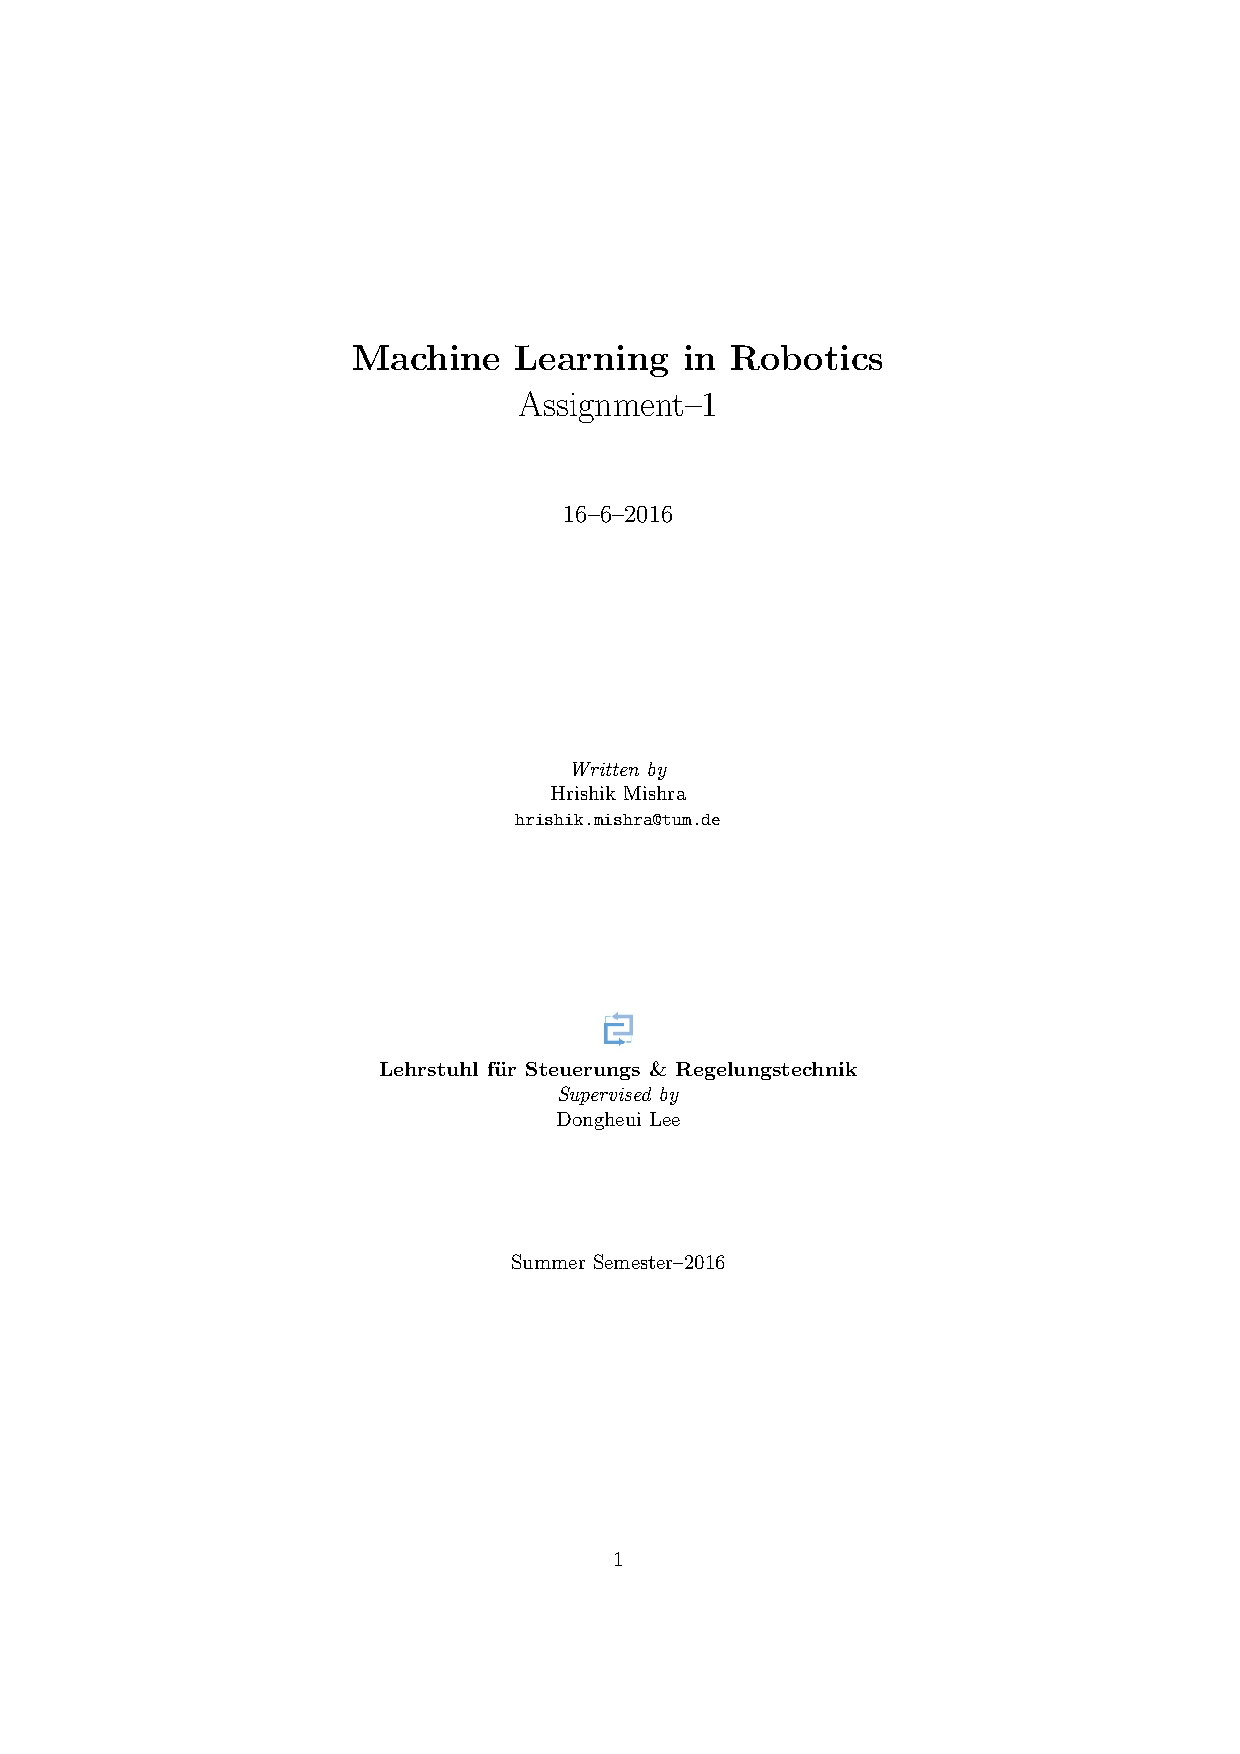
\includepdf{Report_03_titlePage}
\begin{flushleft}
\textbf{Exercise--1:}
\textit{
Estimating velocity motion model of a mobile robot through linear regression.}
\end{flushleft}
Through k-fold cross validation, the model parameters $p_1$ (for position) and $p_2$ (for orientation) were selected which accrued the least estimation errors in position and orientation as given in. \textbf{[1]}
\begin{table}[h!]
\begin{center}
\begin{tabular}{||c|c|c|c|c|c||}
\hline\hline
\textbf{$K$} & \textbf{$p_1$} & \textbf{$p_2$} & \textbf{$param_x$ }& \textbf{$param_y$} & \textbf{$param_{\theta}$} \\[0.5ex]
\hline
\multirow{16}{1em}{$2$} &
\multirow{16}{1em}{$5$} &
\multirow{16}{1em}{$3$} &
$0.00220625732556086$ & $-0.00269493977200706$ & $-0.000595151484125002$ \\
& & &
$0.921732195858891$ & $-0.00135809592112290$ & $-0.000171073749124448$ \\
& & &
$0.00657348550645994$ & $-0.0115383171659957$ & $0.999714709020228$ \\
& & &
$-0.00162656965276813$ & $0.473042321915390$ & $0.000839355025048955$ \\
& & &
$-0.000991575978557237$ & $0.000244539456729993$ & $0.000126866877646434$\\
& & &
$0.00248490664424307$ & $-0.00826729432491700$ & $0.00178272525920989$ \\
& & &
$0.00231358751656282$ & $7.46931348188875e-05$ & $-0.000141046904408991$\\
& & &
$-1.16646541576460e-05$ & $4.38102067757857e-05$ & $-4.52228930367076e-06$\\ & & &
$-0.0130056609219627$ & $0.0164373055385540$ & $-0.000622237972551573$ \\
& & &
$0.000122681135091493$ & $-0.000976996332548495$ & $-1.32208929849420e-05$\\ & & &
$1.28355799646602e-05$ & $-5.28891350696321e-06$ & \\
& & &
$-0.00445663266774616$ & $0.00429852335997573$ &\\
& & &
$-4.30989334269219e-05$ & $-4.41870625680025e-06$ & \\
& & &
$1.66957256114036e-06$ & $-2.69105974566428e-07$ & \\
& & &
$0.00259767597943068$ & $-0.00381272453688410$ & \\
& & &
$-4.02394497236582e-07$ & $2.10157140577462e-06$ &\\



\hline
\multirow{13}{1em}{$5$}  & 
\multirow{13}{1em}{$4$} &
\multirow{13}{1em}{$1$} &
$0.00250438198744831$ & $-0.00432378702432523$ & $0.000807837315929524$ \\
& & & $0.919758171529195$ & $-0.00100147026158884$ & $-0.000319015102912379$\\
& & & $-0.00285535207851188$ & $0.00144804828720765$ & $0.998697948732518$ \\
& & & $-0.000743846577077336$ & $0.467984381559629$ & $0.000321416083203675$ \\
& & & $-0.00103415346607637$ & $0.000568498345337271$ & \\
& & &$0.00137429795052516$ & $-0.00252770680607292$ &\\
& & &$0.00248687885776973$ & $-0.00102513134746683$ &\\
& & & $0.000136005129586935$ & $1.92455105264459e-05$ & \\
& & & $-0.000269081593446607$ & $-0.00167419363591914$ &\\
& & & $6.69261198540723e-05$ & $-0.000672538046125717$ &\\
& & &$1.30609808751867e-05$ & $-7.84620179300530e-06$ &\\
& & &$-0.00428157284345875$ & $0.00347662125530490$ &\\
& & & $-4.51742614704264e-05$ & $8.71551716809008e-06$ &\\
\hline
\end{tabular}
\end{center}
\caption{Simulation results with different k-fold validations}
\end{table}
\clearpage
The visualized dynamics is provided for each of the k-fold parameters below.

\begin{figure}[!ht]
	\graphicspath{{./Exercise1/}}
	\centering
	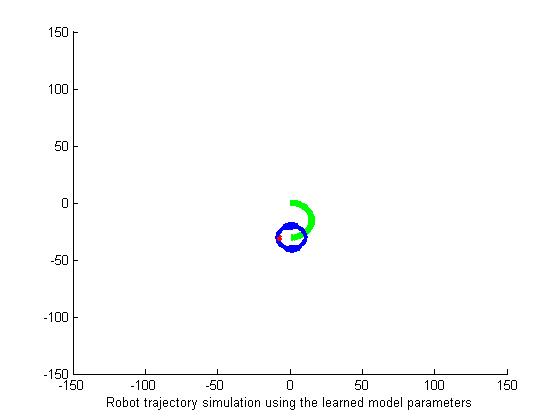
\includegraphics[scale=0.5]{k_2_fig_1}	
	
	\begin{flushleft}
	\caption{Inputs: $v=0.5,\omega=-0.03$, $k=2$}
	\end{flushleft}
	\label{fig:fig_1}
\end{figure}

\begin{figure}[!ht]
	\graphicspath{{./Exercise1/}}
	\centering
	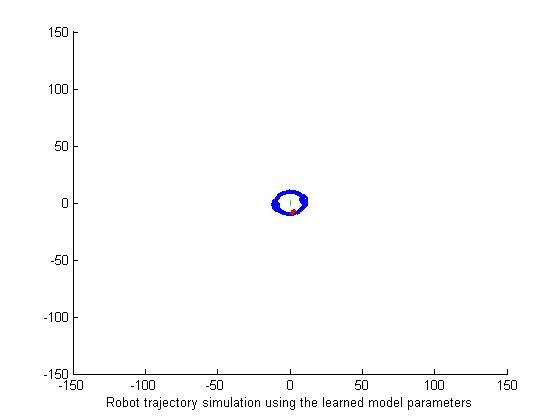
\includegraphics[scale=0.5]{k_2_fig_2}	
	
	\begin{flushleft}
	\caption{Inputs: $v=0,\omega=0.05$, $k=2$}
	\end{flushleft}
	\label{fig:fig_2}
	
\end{figure}

\begin{figure}[!ht]
	\graphicspath{{./Exercise1/}}
	\centering
	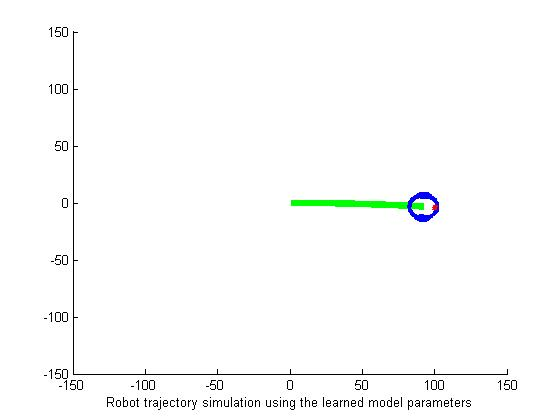
\includegraphics[scale=0.5]{k_2_fig_3}	
	
	\begin{flushleft}
	\caption{Inputs: $v=1,\omega=0$, $k=2$}
	\end{flushleft}
	\label{fig:fig_3}
	
\end{figure}

\begin{figure}[!ht]
	\graphicspath{{./Exercise1/}}
	\centering
	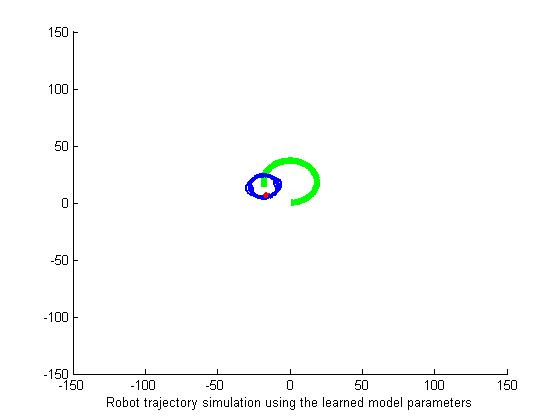
\includegraphics[scale=0.5]{k_2_fig_4}	
	
	\begin{flushleft}
	\caption{Inputs: $v=1,\omega=0.05$, $k=2$}
	\end{flushleft}
	\label{fig:fig_4}
	
\end{figure}

\begin{figure}[!ht]
	\graphicspath{{./Exercise1/}}
	\centering
	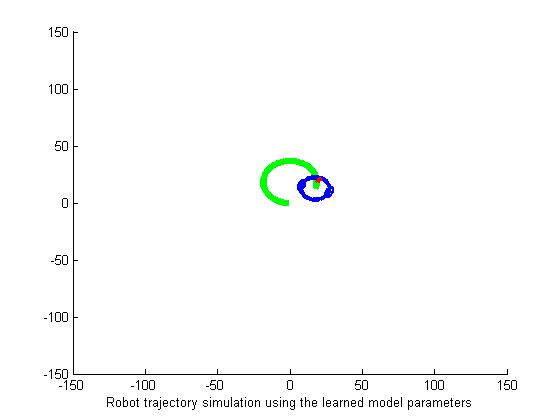
\includegraphics[scale=0.5]{k_2_fig_5}	
	
	\begin{flushleft}
	\caption{Inputs: $v=-1,\omega=-0.05$, $k=2$}
	\end{flushleft}
	\label{fig:fig_5}
	
\end{figure}


\begin{figure}[!ht]
	\graphicspath{{./Exercise1/}}
	\centering
	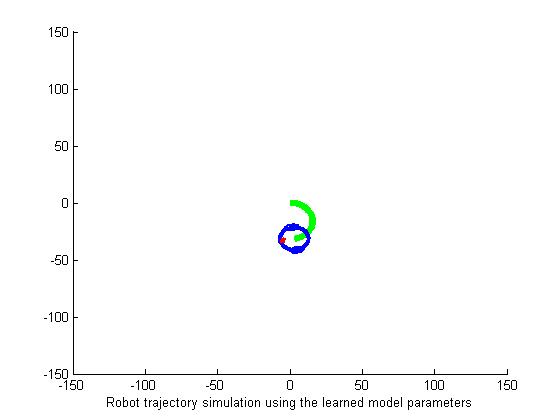
\includegraphics[scale=0.5]{k_5_fig_1}	
	
	\begin{flushleft}
	\caption{Inputs: $v=0.5,\omega=-0.03$, $k=5$}
	\end{flushleft}
	\label{fig:fig_6}
\end{figure}

\begin{figure}[!ht]
	\graphicspath{{./Exercise1/}}
	\centering
	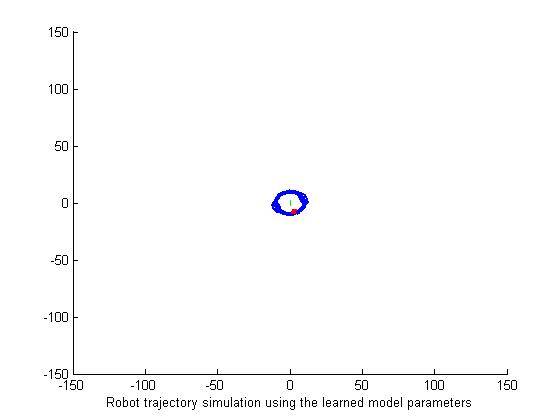
\includegraphics[scale=0.5]{k_5_fig_2}	
	
	\begin{flushleft}
	\caption{Inputs: $v=0,\omega=0.05$, $k=5$}
	\end{flushleft}
	\label{fig:fig_7}
	
\end{figure}

\begin{figure}[!ht]
	\graphicspath{{./Exercise1/}}
	\centering
	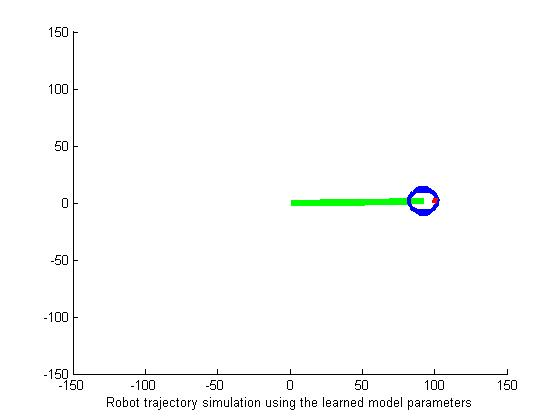
\includegraphics[scale=0.5]{k_5_fig_3}	
	
	\begin{flushleft}
	\caption{Inputs: $v=1,\omega=0$, $k=5$}
	\end{flushleft}
	\label{fig:fig_8}
	
\end{figure}

\begin{figure}[!ht]
	\graphicspath{{./Exercise1/}}
	\centering
	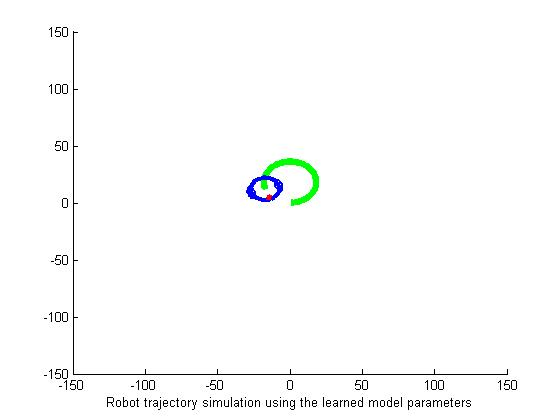
\includegraphics[scale=0.5]{k_5_fig_4}	
	
	\begin{flushleft}
	\caption{Inputs: $v=1,\omega=0.05$, $k=5$}
	\end{flushleft}
	\label{fig:fig_9}
	
\end{figure}

\begin{figure}[!ht]
	\graphicspath{{./Exercise1/}}
	\centering
	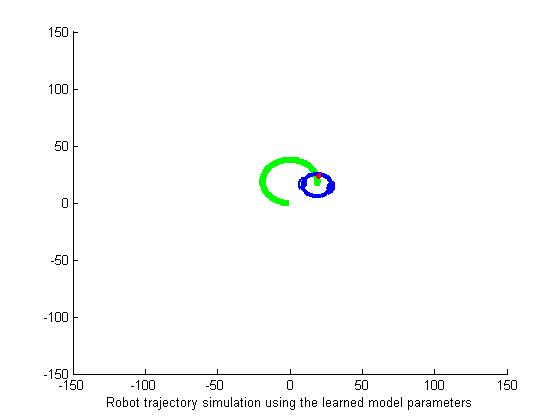
\includegraphics[scale=0.5]{k_5_fig_5}	
	
	\begin{flushleft}
	\caption{Inputs: $v=-1,\omega=-0.05$, $k=5$}
	\end{flushleft}
	\label{fig:fig_10}
	
\end{figure}

\clearpage
\textbf{Exercise--2:}
\textit{Handwritten digits classification using Bayesian classifier.}\\
The parameter \textbf{$d$} is the complexity of the Principal Component Analysis (PCA) model. In this simulation, the value of \textbf{$d$} was changed from $1$ to $60$ in steps of $2$. Figure \ref{fig:fig_11} shows the classification errors as a function of the eigen depth, \textbf{$d$}. Based on the figure, it can be inferred that the optimal value for \textbf{$d$} is $25$ and the total classification error is $4.27\%$. Also, based on data provided in \textbf{[1]},the \textbf{$d$} value of $15$ results in an error of $7.03\%$ \\


\begin{figure}[!ht]
	\graphicspath{{./Exercise2/}}
	\centering
	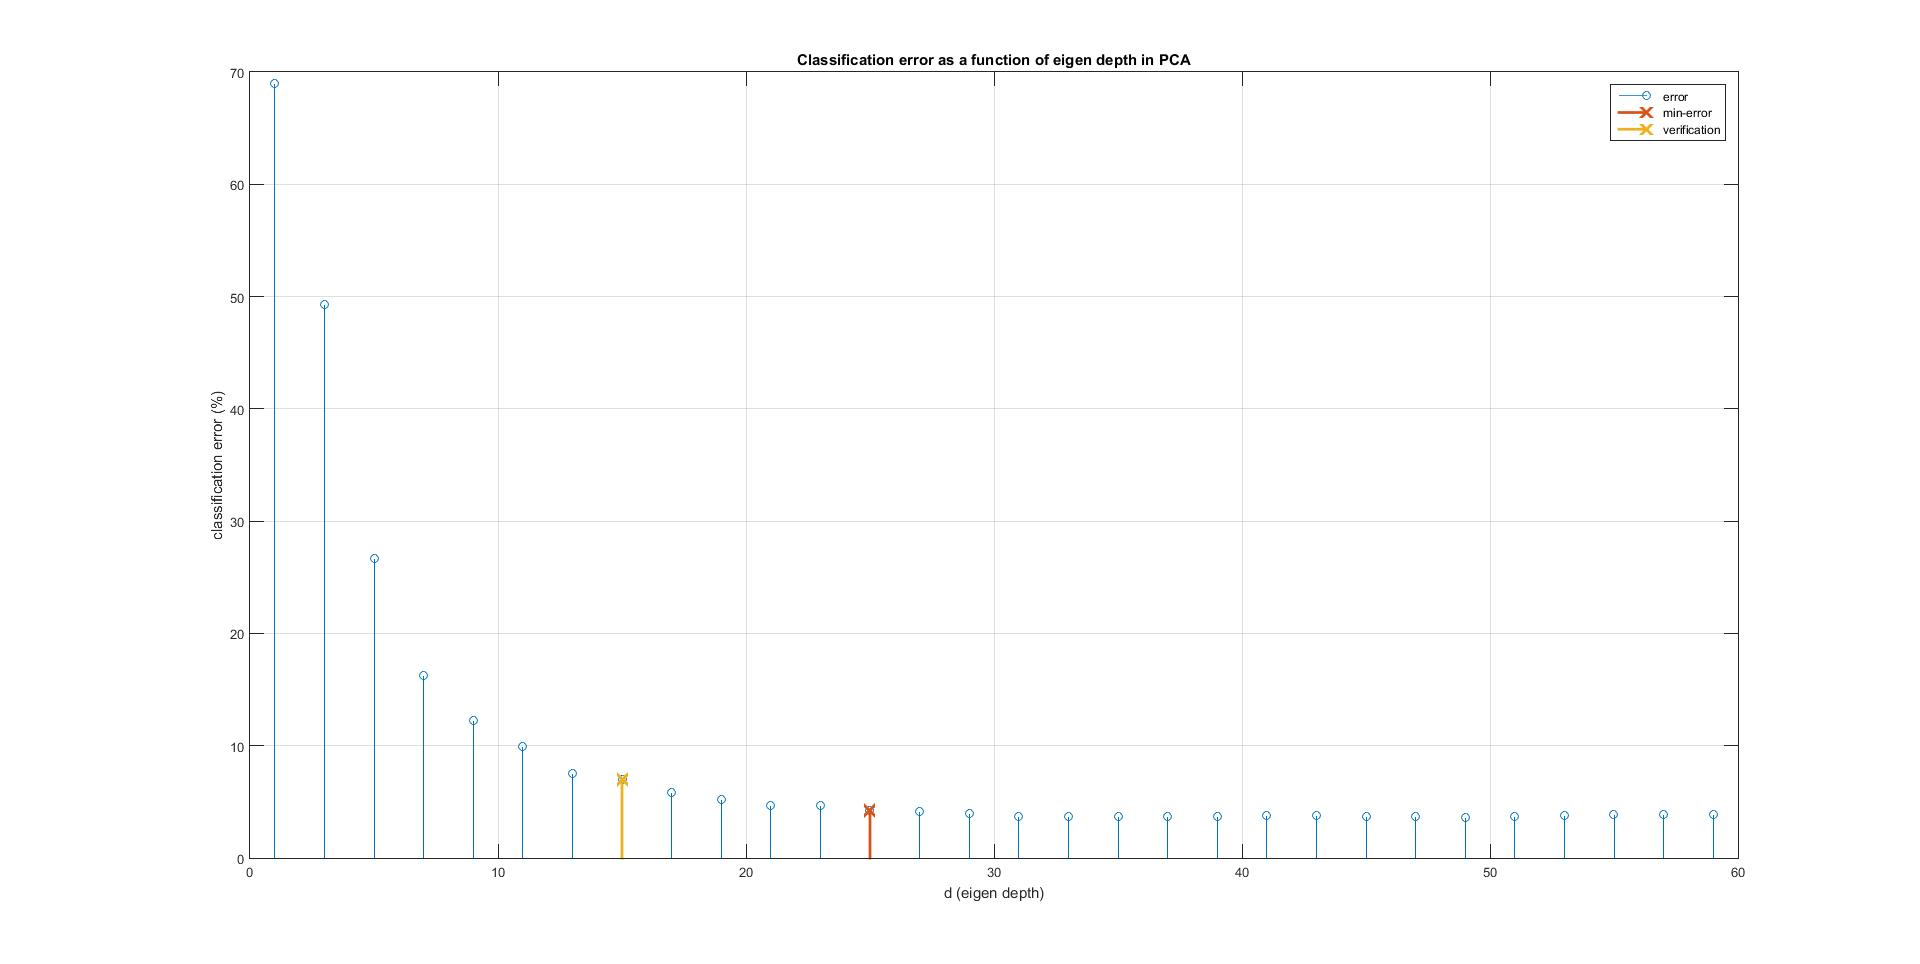
\includegraphics[scale=0.21]{ErrorAsFunction_d}	
	
	\begin{flushleft}
	\caption{Classification error as function of eigen depth in PCA}
	\end{flushleft}
	\label{fig:fig_11}
	
\end{figure}

The confusion matrix as given by the \emph{MATLAB} function \texttt{confusionmat} for $\textbf{$d$}=25$ is,

\[\left[ \begin{array}{cccccccccc}
968 &	0 &	2 &	0 &	0 &	5 &	1 &	1 &	3 &	0\\
0 &	1103 &	6 &	 4 &	0 &	1 &	3 &	0 &	17 &	1\\
5 &	0 &	1003 &	4 &	2 &	0 &	4 &	1 &	13 &	0\\
0 &	0 &	7 &	970 &	1 &	10 &	0 &	6 &	12 &	4\\
1 &	0 &	6 &	0 &	954 &	0 &	1 &	2 &	2 &	16\\
4 &	0 &	1 &	22 &	0 &	855 &	2 &	0 &	6 &	2\\
18 &	1 &	1 &	0 &	2 &	14 &	917 &	0 &	5 &	0\\
0 &	5 &	30 &	1 &	6 &	6 &	0 &	946 &	12 &	22\\
4 &	0 &	7 &	21 &	1 &	5 &	3 &	3 &	918 &	12\\
4 &	3 &	10 &	8 &	19 &	3 &	0 &	6 &	17 &	939\\
\end{array} \right]\]
\\
The total number of successfully classified digits were $9573$. From the confusion matrix, we can infer that $6$ quite often (\textit{22 times}) gets classified as $4$, and $9$ gets classified as $8$ and misclassified instead of $2$ as often (\textit{17 times}).

\clearpage
\textbf{Exercise--3:}
\textit{Human motion clustering.}\\
The motion data available was passed through two different classification algorithms, k-means and non-uniform Binary split. Figure 12 \ref{fig:fig_12} demonstrates the classification of the 3-d motion points in an XY-view for the letters \emph{l}, \emph{o} and \emph{x}. As required in \textbf{[1]}, the convergence of the k-means algorithm to a \emph{decrement} of the \textbf{distortion} function could not be reached to $10^{-6}$ since the computing was taking an inordinate amount of time. The results shown aforementioned are computed with a \emph{decrement} of $10^3$. 
\begin{figure}[!ht]
	\graphicspath{{./Exercise3/}}
	\centering
	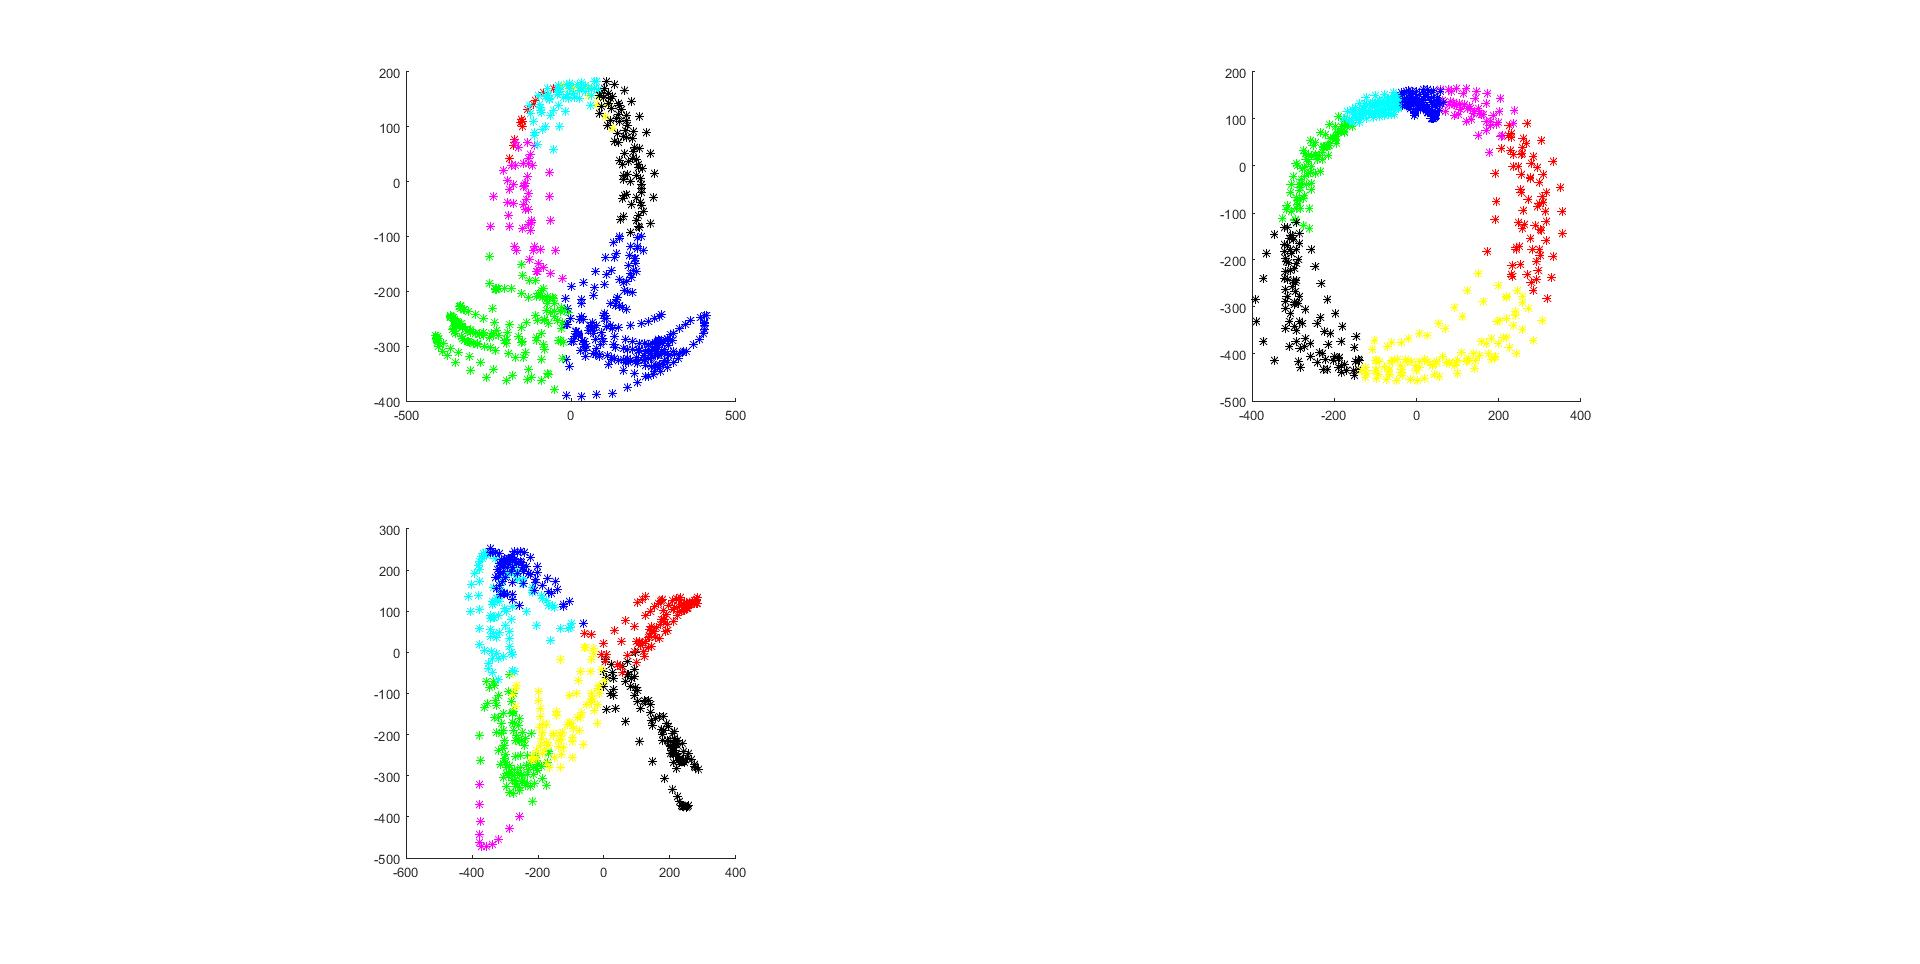
\includegraphics[scale=0.15]{k_means}	
	
	\begin{flushleft}
	\caption{K-means clustering with $k=7$}
	\end{flushleft}
	\label{fig:fig_12}
	
\end{figure}


Similarly, the results of classification are shown in Figure 13 \ref{fig:fig_13}. From the result, it was inferred that the \emph{non-uniform Binary split} algorithm's classification is largely dependent on the infinitesimally small vector which, in this case, was specified in \textbf{[1]}.

\begin{figure}[!ht]
	\graphicspath{{./Exercise3/}}
	\centering
	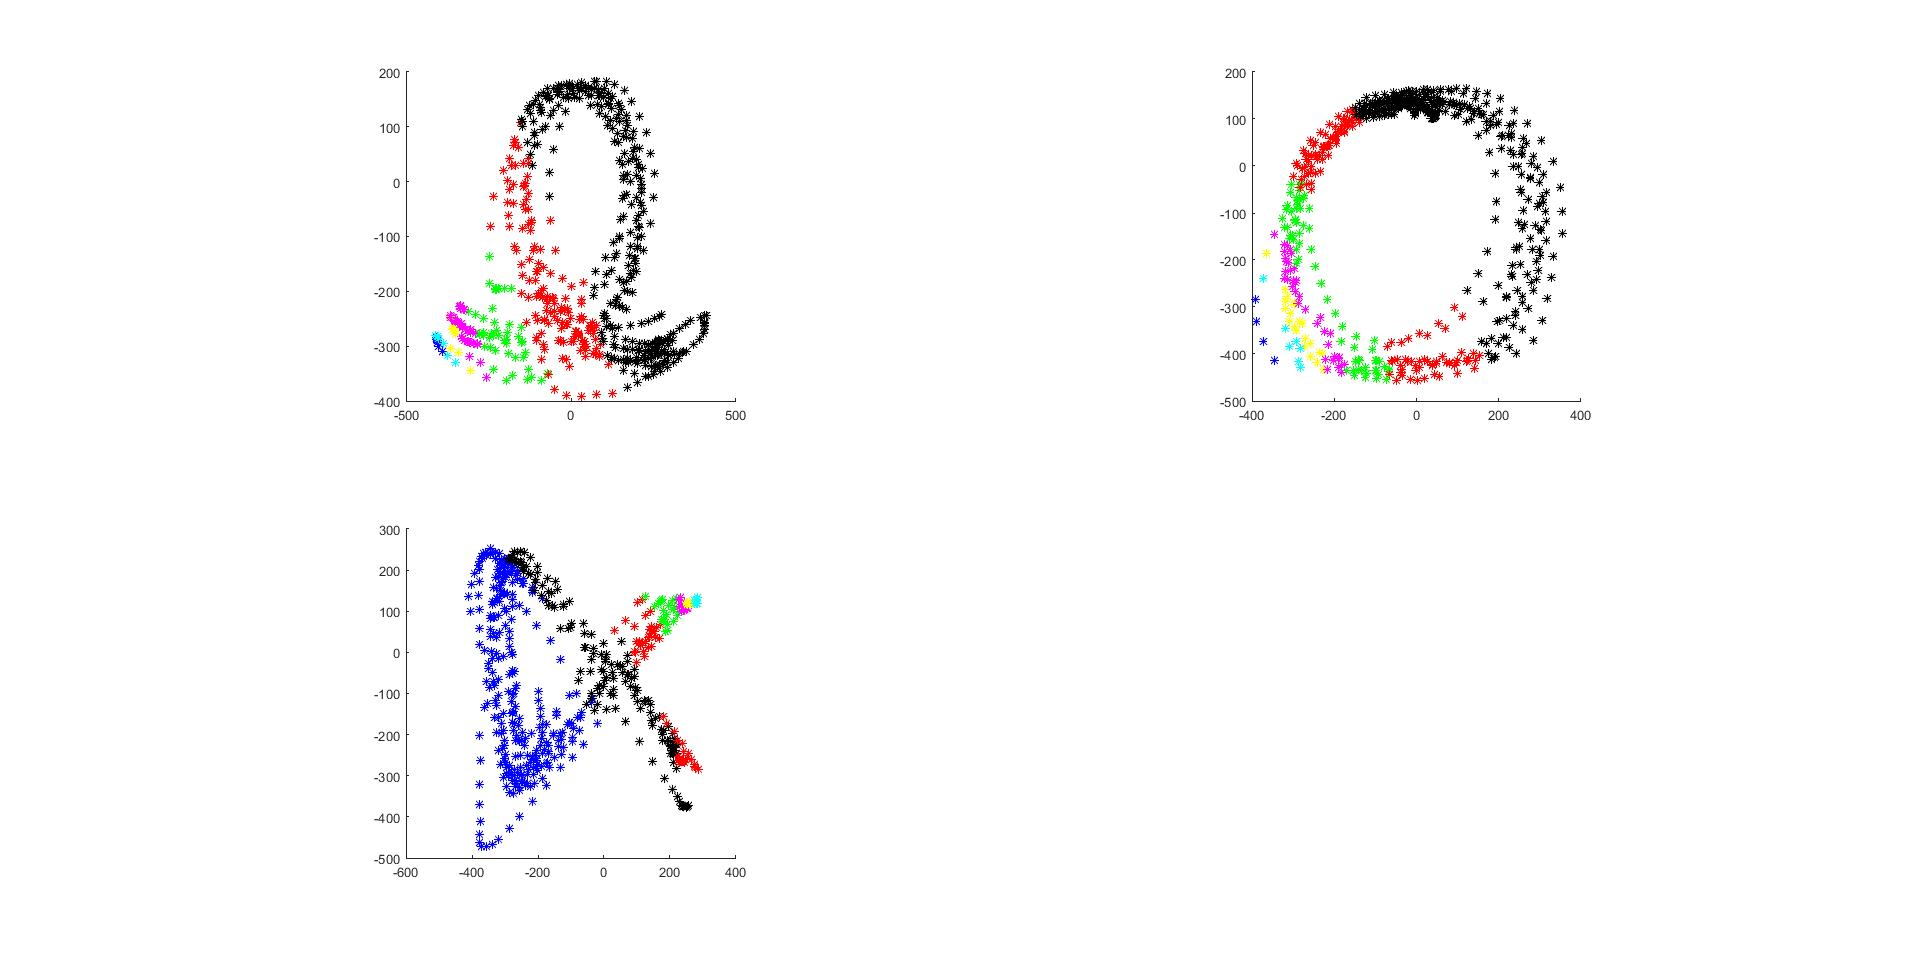
\includegraphics[scale=0.15]{nubf}	
	
	\begin{flushleft}
	\caption{non-uniform binary clustering with $k=7$}
	\end{flushleft}
	\label{fig:fig_13}
	
\end{figure}

\clearpage
\begin{center}
	\textbf{\large{References}}\\
\end{center}
[1]. Assignment1.pdf, Prof. Dongheui Lee, Lehrstuhl f\"ur STEUERUNGS-
\& REGELUNGSTECHNIK, Machine Learning in Robotics.




\end{document}